\documentclass{article}
\usepackage{graphicx} % Required for inserting images
\usepackage{minted}
\title{Digital Clock}
\author{Pothuri Rahul - EE24BTECH11050}
\date{ }

\begin{document}

\maketitle

\section{Introduction}
This project presents a digital clock using an Arduino Uno, a 7447 BCD to 7-segment decoder IC, and six common cathode 7-segment displays. The clock is designed to display time in HH:MM:SS format. It utilizes multiplexing to control all displays using a single 7447 IC. The Arduino manages time updates and ensures proper digit transitions. The clock runs in real-time and resets after 24 hours. This project demonstrates the practical implementation of BCD to 7-segment conversion and multiplexing in digital electronics.


\section{Hardware things}
\subsection{Components used :} 
\begin{itemize}
\item Breadboard
\item 744 IC (BCD to 7 segment converter)
\item Six 7 segment display
\item Arduino board
\item Connecting cables and wires
\item Mobile
\end{itemize}
\subsection{Circuit design} 
\subsubsection{7447 to Arduino}
These are the following connections I made between 7447 IC and Arduino

\begin{center}
    \begin{tabular}{|c|c|}
        \hline
        \textbf{7447} & \textbf{ARDUINO} \\
        \hline
        A (pin 7) & 2 \\
        \hline
        B (pin 1) & 3 \\
        \hline
        C (pin 2) & 4 \\
        \hline
        D (pin 6) & 5 \\
        \hline
        $V_{cc}$ (pin 16) & 5 V \\
        \hline 
        GND (pin 8) & GND \\
        \hline
    \end{tabular}
\end{center}
\subsubsection{7447 to 7 segment display}
Following connections are to be done between the 7447 and all six 7 - segment displays.

\begin{center}
    \begin{tabular}{|c|c|}
    \hline
    \textbf{7447}& \textbf{7 segment display}  \\
    \hline
    a (pin 13)& a \\
    \hline
    b (pin 12)& b \\
    \hline
    c (pin 11)& c \\
    \hline
    d (pin 10) & d \\
    \hline
    e (pin 9) & e \\
    \hline 
    f (pin 15) & f \\
    \hline 
    g (pin 14) & g \\
    \hline
    \end{tabular}
\end{center}
Actually we use six 7 segment displays to get HH:MM:SS format. let us consider $H_1$ display is tens of hours , $H_2$ display is ones of hours , $M_1$ display is tens of minutes , $M_2$ display is ones of minutes , $S_1$ display is tens of seconds and $S_2$ display is ones of seconds.

We use the multiplexing technique to control six displays with a single 7447 IC.For that let us connect the com 7 segment displays to Arduino and GND pins of 7 segment displays to ground .

\begin{center}
\begin{tabular}{|c|c|c|}
    \hline
    \textbf{Display} & \textbf{Pin} & \textbf{Arduino pin} \\
    \hline
    $S_2$ & COM & 6 \\
    \hline
    $S_1$ & COM & 7 \\
    \hline
    $M_2$ & COM & 8\\
    \hline
    $M_1$ & COM & 9 \\
    \hline
    $H_2$ & COM & 10\\
    \hline
    $H_1$ & COM & 11 \\
    \hline
\end{tabular}
\end{center}


\section{Software things}
\subsection{Code used}
The cpp code used is the following
\begin{minted}[frame=lines, linenos, fontsize=\footnotesize]{c}
// 7447 BCD input pins
const int A = 2, B = 3, C = 4, D = 5;
// Display common pins
const int digits[] = {11, 10, 9, 8, 7, 6};

int hours = 17, minutes = 7, seconds = 5;
unsigned long prevMillis = 0;
const int interval = 1000;  // Update time every 1 second

void setup() {
    Serial.begin(9600);

    // Set up 7447 BCD pins as output
    for (int i = A; i <= D; i++) {
        pinMode(i, OUTPUT);
        digitalWrite(i, LOW);
    }

    // Set up display common pins as output
    for (int i = 0; i < 6; i++) {
        pinMode(digits[i], OUTPUT);
        digitalWrite(digits[i], HIGH);  // Start with all displays OFF
    }

    Serial.println("Clock Started!");
}

void loop() {
    unsigned long currentMillis = millis();

    // Update time every second
    if (currentMillis - prevMillis >= interval) {
        prevMillis = currentMillis;
        updateClock();
        Serial.print("Time: ");
        Serial.print(hours); Serial.print(":");
        Serial.print(minutes); Serial.print(":");
        Serial.println(seconds);
    }

    // Refresh the display continuously
    multiplexDisplay();
}

void updateClock() {
    seconds++;
    if (seconds == 60) {
        seconds = 0;
        minutes++;
        if (minutes == 60) {
            minutes = 0;
            hours++;
            if (hours > 24) hours = 0;
        }
    }
}

void multiplexDisplay() {
    for (int i = 0; i < 6; i++) {
        int digitValue = getDigit(i);
        showDigit(digitValue, i);
    }
}

void showDigit(int num, int digitIndex) {
    turnOffDisplays();  
    digitalWrite(digits[digitIndex], HIGH);  // Activate display
    set7447(num);  
    delay(5);  // Small delay to allow visibility
    digitalWrite(digits[digitIndex], LOW); // Turn off display
}

void set7447(int num) {
    digitalWrite(A, num & 1);
    digitalWrite(B, (num >> 1) & 1);
    digitalWrite(C, (num >> 2) & 1);
    digitalWrite(D, (num >> 3) & 1);
}

void turnOffDisplays() {
    for (int i = 0; i < 6; i++) {
        digitalWrite(digits[i], LOW);  // Turn off all displays
    }
}

int getDigit(int index) {
    switch (index) {
        case 0: return hours / 10;    
        case 1: return hours % 10;    
        case 2: return minutes / 10;  
        case 3: return minutes % 10;  
        case 4: return seconds / 10;  
        case 5: return seconds % 10;  
        default: return 0;
    }
}
\end{minted}
\textbf{Reference :} Used some AI Tools like chat-gpt for getting the code.
\subsection{Explanation of the code}

The given Arduino code implements a digital clock (HH:MM:SS) using a 7447 BCD to 7-segment decoder with multiplexing.

\subsubsection{Key Features}
\begin{itemize}
    \item \textbf{Pin Definitions:}  
    \begin{itemize}
        \item \texttt{A, B, C, D} → BCD input pins for 7447.
        \item \texttt{digits[]} → Stores the 6 display common pins.
    \end{itemize}
    \item \textbf{Time Variables:}  
    \begin{itemize}
        \item \texttt{hours, minutes, seconds} → Stores current time.
        \item \texttt{prevMillis, interval} → Tracks updates every 1 second.
    \end{itemize}
    \item \textbf{\texttt{setup()}:} Initializes serial communication and sets display pins OFF.
    \item \textbf{\texttt{loop()}:} 
    \begin{itemize}
        \item Updates time every second using millis().
        \item Calls \texttt{multiplexDisplay()} to refresh the 7-segment display.
    \end{itemize}
    \item \textbf{\texttt{updateClock()}:} Increments seconds, minutes, and hours like a real clock.
    \item \textbf{\texttt{multiplexDisplay()}:} Switches between six digits rapidly using multiplexing.
    \item \textbf{\texttt{showDigit(num, digitIndex)}:}  
    \begin{itemize}
        \item Turns off all displays.
        \item Activates the required digit.
        \item Sends the corresponding BCD number to the 7447 decoder.
    \end{itemize}
    \item \textbf{\texttt{set7447(num)}:} Converts the digit to BCD format for the 7447 IC.
    \item \textbf{\texttt{turnOffDisplays()}:} Turns off all displays to prevent ghosting.
    \item \textbf{\texttt{getDigit(index)}:} Extracts individual digits from HH:MM:SS.
\end{itemize}

\subsubsection{How it Works}
\begin{itemize}
    \item Uses multiplexing to display six digits using one 7447 IC.
    \item millis() ensures time updates every second without delay(), allowing smooth display refresh.
    \item The method is power-efficient, simple, and can scale to a full digital clock with minimal hardware.
\end{itemize}
\section{Working process }

\begin{itemize}
\item The Arduino tracks the time (seconds, minutes, hours) using the millis() function.
\item The time values are converted into BCD format and sent to the 7447 decoder IC.
\item The 7447 IC drives the 7-segment displays according to the BCD input.
\item Multiplexing technique is used to control six displays with a single 7447 IC.
\item The display updates every second, ensuring proper timekeeping.
\item The clock resets to 00:00:00 after reaching 24:00:00.
\end{itemize}

\begin{figure}[H]
    \centering
    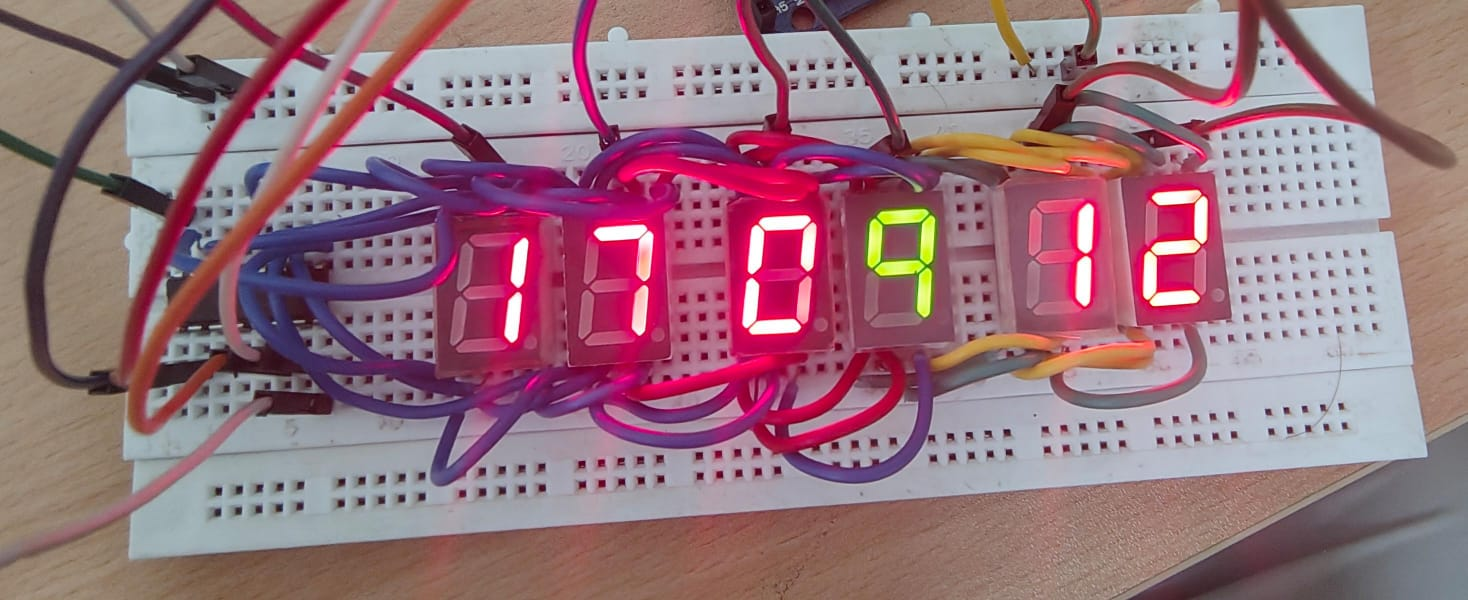
\includegraphics[width=0.5\linewidth]{WhatsApp Image 2025-03-22 at 9.20.31 PM.jpeg}
    \caption{Clock made showing the time 17:09:12}
\end{figure}

\section{Future Enhancements}
\begin{itemize}
\item Using Real - Time Clock (RTC) would be better since we can get the real-life time even when their is no power is given to arduino.
\item Adding push buttons to set buttons will be useful.
\item Some gets habituated to 12 -  hours formart , for them it would be useful to add another display to mention AM and PM.
\item We can make an alarm using a buzzer and little changes in code.
\item Instead of 7 segment display , we can also use LED display so that we can add some more features like Date, Temperature by making some changes in the code and using some other sensors to measure the temperature.
\end{itemize}

\section{Conclusion}

By doing this project I learned the usage of 7447 , 7 segment display and multiplexing. This project successfully implemented a fully functional digital clock using an Arduino Uno, a 7447 decoder, and six 7-segment displays. The use of multiplexing allowed efficient control of the displays with a single decoder IC .


\end{document}
